\subsection{Systems Biology Simulations using the WESTPA/BNG Plugin}

\subsubsection{Introduction}
This tutorial focuses on a scenario in systems biology in which the WE strategy can be useful: enhanced sampling of rare events in a non-spatial model. 
Here we focus on a BioNetGen language (BNGL) rule-based model for a biological signaling network that consists of a set of structured molecule types and a set of rules that define the interactions between the molecule types. 
While the average steady-state behavior of the model can be obtained using ordinary differential equations, the full kinetics of the model can only be obtained from stochastic simulations. 
However, adequate sampling of any rare events in the model can be a challenge for stochastic simulations. 
In this tutorial, we will use WESTPA to orchestrate BNGL simulations that are propagated by the BNG software package. 
As mentioned above, WESTPA is interoperable with any stochastic dynamics engine, including the BNG software.

\textbf{Learning objectives.} We will simulate a BNGL rule-based model of a two-gene switch motif that exhibits mutually exclusive activation and inhibition.
Specific learning objectives include:
\begin{enumerate}
    \item How to install the WESTPA/BNG plugin and set up a WESTPA/BNG simulation; 
    \item How to apply adaptive Voronoi binning, which can be used for both non-spatial and molecular systems; 
    \item How to run basic analyses tailored for high-dimensional WESTPA/BNG simulations.
\end{enumerate} 

\subsubsection{Prerequisites}
Users should have a working knowledge of BNGL models ({\url{http://bionetgen.org}}) and the WESTPA 2.0 software package. 
This tutorial will make use of the WEBNG Python package, which facilitates the integration of WESTPA with the BNG software and requires Python 3.7 or later versions. 
To install the WEBNG package: 

\begin{verbatim}
  $ git clone 
        https://github.com/ASinanSaglam/webng.git
  $ python -m pip install -e .
\end{verbatim}

For common installation issues, see {\url{https://webng.readthedocs.io/en/latest/quickstart.html#installation}}. Alternatively the user can use a Docker container where the environment is already prepared correctly using the command: 
\begin{verbatim}
  $ docker pull 
          ghcr.io/westpa/westpa2_tutorials:webng
\end{verbatim}

Note that this requires a Docker installation, for more information see Docker documentation ({\url{https://docs.docker.com/get-docker}}). 
Once the docker image is downloaded, you can run the image with:
\begin{verbatim}
  $ docker run -it --entrypoint /bin/bash 
            ghcr.io/westpa/westpa2_tutorials:webng
\end{verbatim}

\textbf{Computational requirements.} This tutorial requires \textasciitilde500 MB disk space. 
The simulation takes at most 1 hour of wall-clock time using a single CPU core of a 3.2GHz Intel Core i7 processor. 
We recommend using the \verb|WEBNG| package on a Unix system. 
While the package has not been tested on Windows systems, one can try using the Windows subsystem for Linux (WSL; {\url{https://docs.microsoft.com/en-us/windows/wsl/install}}).

\subsubsection{Setting up the simulation}

\noindent\textbf{The model.} Our BNGL model consists of two genes, gene A and gene B, that are transcribed to produce proteins A and B, respectively. 
Protein A binds to the gene A promoter site to activate protein A production and to the gene B promoter site to repress B production. 
Likewise, protein B activates gene B and represses gene A. 
The two most populated states therefore consist of either (1) high quantities of protein A and low quantities of protein B, or (2) high quantities of protein B and low quantities of protein A. 
Transitions between these two states are rare events. 

\begin{figure}[t]
\centering
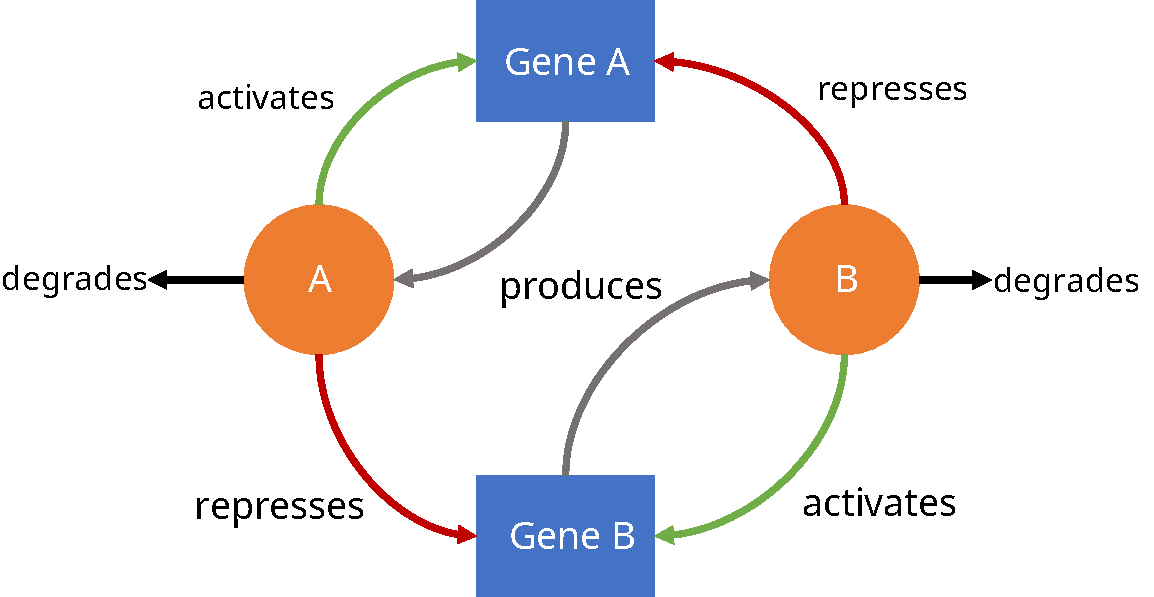
\includegraphics[width=\columnwidth]{figures/Figure13_Network.pdf}
\caption{Two-gene network of exclusive mutual inhibition and self activation.}
\end{figure}

\textbf{Preparing the simulation environment.} For this portion of the tutorial, you can use either your own BNGL model or the ExMISA model described above, which is the default WEBNG example. 
WEBNG uses a YAML configuration file to set up a WESTPA folder. 
The \verb|WEBNG template| subcommand gives you a YAML config file with the same defaults which you can then edit and use to generate the WESTPA simulation folder. 

If you are using the default example, the command to generate the template is the following:
\begin{verbatim}
  $ webng template -o mysim.yaml 
\end{verbatim}

If you are using your own model file called \verb|exmisa.bngl|, the command is:
\begin{verbatim}
  $ webng template -i exmisa.bngl -o mysim.yaml
\end{verbatim}

This command will generate the YAML file, \verb|mysim.yaml|. For the full set of configuration options, see {\url{https://webng.readthedocs.io/en/latest/config.html}}. 
Path options are specified automatically using the libraries that are already installed. 
Propagator options will also be automatically populated according to the BNGL model. 
By default, this simulation setup will use an adaptive Voronoi binning scheme \citep{zhang_exact_2010} due to the fact that rectilinear binning is not feasible for high-dimensional BNG models. 
The \verb|center_freq| option sets the frequency of Voronoi bin addition, in units of WE iterations, \verb|max_centers| is the maximum number of Voronoi bins that will be added, \verb|traj_per_bin| is the number of trajectory walkers per Voronoi bin, and \verb|max_iter| option sets the maximum number of WE iterations. 
All of these options can be modified after the simulation folder is set up (see {\url{https://github.com/westpa/westpa/wiki/User-Guide#Setting_Up_a_WESTPA_Simulation}}). 

By default, the stochastic simulator is set to libroadrunner ({\url{http://libroadrunner.org}}). 
To use this simulator, we must first convert the BNGL model to a systems biology markup language (SBML) model. 
Next, we use the WEBNG software to compile the SBML model into a Python object, which allows for efficient simulation of the model. 
WEBNG also supports the use of the \verb|BNG| simulation package. 
However, the use of this package will result in higher file I/O operations. 
Any other stochastic simulator will require the use of a custom WESTPA propagator.

\subsubsection{Running the WE simulation}
To run the simulation, we first need to generate a WESTPA folder using the YAML configuration file generated in the previous step:

\begin{verbatim}
  $ webng setup --opts mysim.yaml
\end{verbatim}

The above command will use the path option \verb|sim_name| as the WESTPA folder, which is automatically set to the model name in the folder you ran the template command. 
Next, we initialize the simulation and run the model in a serial mode using a single CPU: 

\begin{verbatim}
  $ cd exmisa
  $ ./init.sh
  $ w_run --serial
\end{verbatim}

To run the model in a parallel mode using multiple CPU cores, please refer to WESTPA documentation for options available with the \verb|w_run| command-line tool.
The resulting simulation can be found in the \verb|exmisa/| folder directory.

\begin{figure}[t]
\centering
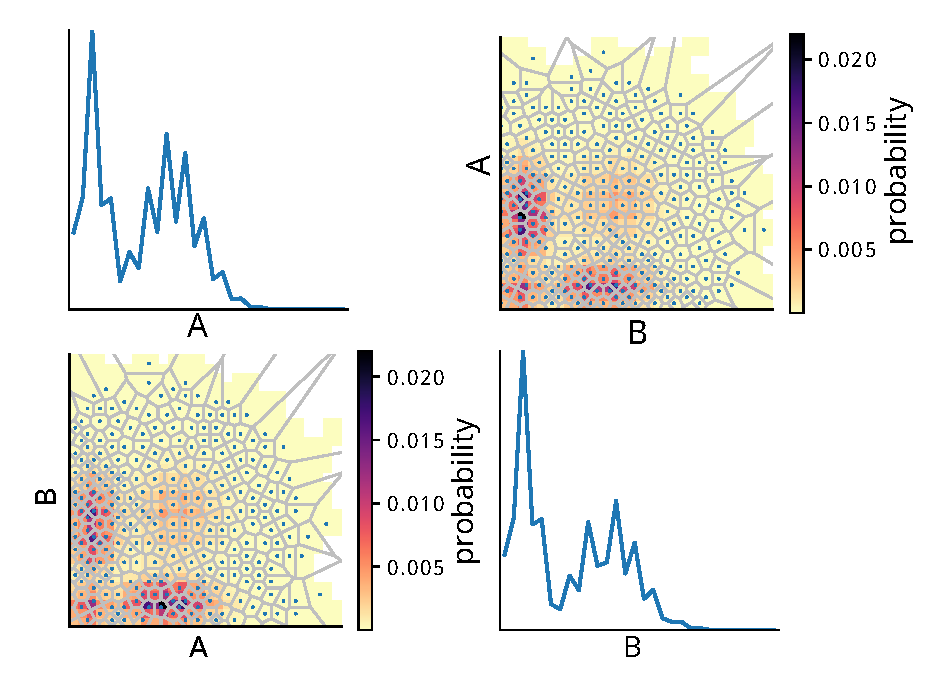
\includegraphics[width=\columnwidth]{figures/Figure14_ProbDist.pdf}
\caption{Probability distributions as a function of the two-dimensional progress coordinate (off-diagonal) and each dimension of the progress coordinate (diagonal).
Grey lines in each off-diagonal plot delineate adaptive Voronoi bins used during the WE simulation.}
\end{figure}

\begin{figure}[t]
\centering
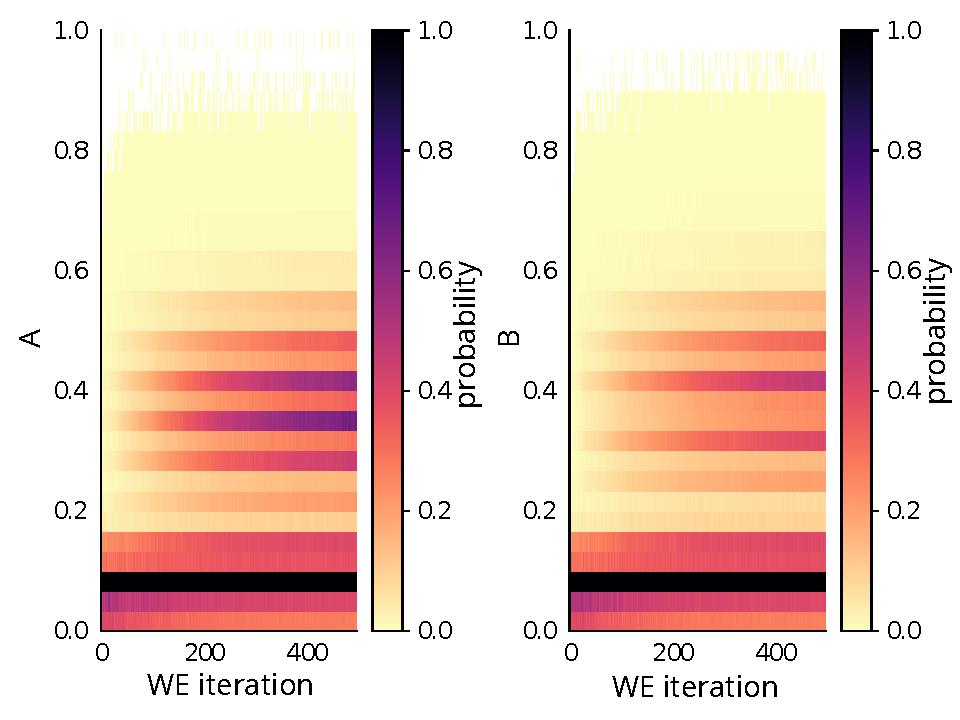
\includegraphics[width=\columnwidth]{figures/Figure15_ProbDist2.pdf}
\caption{Probability distributions of each observable (A or B) of the two-dimensional progress coordinate as a function of WE iteration. 
The striped nature of the distributions is due to the fact that A and B are discrete as opposed to continuous observables.}
\end{figure}

\subsubsection{Analyzing the WE simulation}
To analyze the simulation, we will use the WEBNG package. 
To begin, we edit the YAML file under the folder that contains the configuration file \verb|mysim.yaml|, setting \verb|analyses.enable|, \verb|analyses.average.enable|, and \verb|analyses.evolution.enable| to \verb|True|; and \verb|analyses.average.first-iter| to the simulation half point (default: 50). 
To run the analysis, we use the following command: 

\begin{verbatim}
  $ webng analysis --opts mysim.yaml
\end{verbatim}

The above command will generate an \verb|analysis/| folder in the simulation folder, run the analyses, and generate associated figures. 

By default, \verb|average.png| provides an N$\times$N matrix of plots of the average two-dimensional probability distributions of each observable (dimension) of the WE progress coordinate and each of the other observables. 
The \verb|evolution.png| file gives the time-evolution (number of WE iterations) of probability distributions for each observable and can be used to assess the convergence of simulation, making modifications to the binning scheme if necessary. 


The average two-dimensional probability distributions reveal a total of four states: a low A/low B state, the symmetric low A/high B state and high A/low B states, and a high A/high B state. 
The fourth state is the least probable while the first three states are all highly probable. 
Transitions from low A/high B to high A/low B states are difficult to sample and transitions from low A/high B to high A/high B states are even more difficult to sample. 
The WE algorithm allows the user to sample these states and transitions between the states. 
All analyses should be based on the portion of the simulation that is done evolving. 
If the simulation is still evolving, we recommend extending the simulation until the observables of interest are reasonably converged. 

\subsubsection{Conclusion}

As demonstrated by this tutorial, the WEBNG Python package provides a framework for applying the WESTPA 2.0 software package to BNGL models with minimal user input and simplified installation. 
The adaptive Voronoi binning scheme enables efficient application of high-dimensional progress coordinates for both molecular and non-spatial systems.
Voronoi bins can be effective for exploratory simulations, placing bins as far away as possible from previous bins to inform the creation of a custom binning scheme for sampling the rare-event process of interest. 
However, such bins may not be as effective for surmounting barriers (e.g., compared to the MAB scheme \citep{torrillo_minimal_2021}), as demonstrated by the probability distribution as a function of the WE progress coordinate where many bins near the edges of the configurational space are occupied, but are not of interest. 
Future work with WEBNG will include more detailed analysis options such as automated clustering, generation of networks from bins and clusters, and the estimation of rate constants for transitions between the clusters. 